% !TEX TS-program = lualatex
\documentclass[tikz, border=2mm]{standalone}

\usepackage{fontspec}
\IfFontExistsTF{Times New Roman}{
  \setmainfont{Times New Roman}
}{
  \setmainfont{Liberation Serif}
}
\IfFontExistsTF{Courier New}{
  \setmonofont{Courier New}[Scale=MatchLowercase]
}{}

\usepackage{pgfplots}
\pgfplotsset{compat=1.18}
\usetikzlibrary{shapes.geometric, arrows.meta, positioning, fit, backgrounds, calc}

\begin{document}

% Biểu đồ 1: Tổng số Commits
\begin{tikzpicture}
        \begin{axis}[
            ybar,
            symbolic x coords={phucpt, truongtm, vint, kiennt, thaidg},
            xtick=data,
            nodes near coords,
            nodes near coords align={vertical},
            ylabel={Số lượng Commits},
            xlabel={Thành viên nhóm (PIC)},
            ymin=0, ymax=180,
            bar width=20pt,
            width=14cm, height=6.5cm,
            enlarge x limits=0.15,
            title={\textbf{Tổng số Commits theo từng PIC}}
        ]
        \addplot[fill=blue!40] coordinates {
            (phucpt, 156) 
            (truongtm, 53) 
            (vint, 11) 
            (kiennt, 7) 
            (thaidg, 6)
        };
        \end{axis}
\end{tikzpicture}

% Biểu đồ 2: Tổng số nhánh
\begin{tikzpicture}
        \begin{axis}[
            ybar,
            symbolic x coords={truongtm, phucpt, vint, thaidg, kiennt},
            xtick=data,
            nodes near coords,
            ylabel={Số lượng nhánh đã tạo},
            ymin=0, ymax=10,
            bar width=20pt,
            width=14cm, height=5.5cm,
            enlarge x limits=0.15,
            title={\textbf{Tổng số Nhánh làm việc theo PIC}}
        ]
        \addplot[fill=teal!60] coordinates {
            (truongtm, 8) 
            (phucpt, 6) 
            (vint, 2) 
            (thaidg, 2) 
            (kiennt, 1)
        };
        \end{axis}
\end{tikzpicture}

% Biểu đồ 3: Biểu đồ tròn - Đóng góp Code
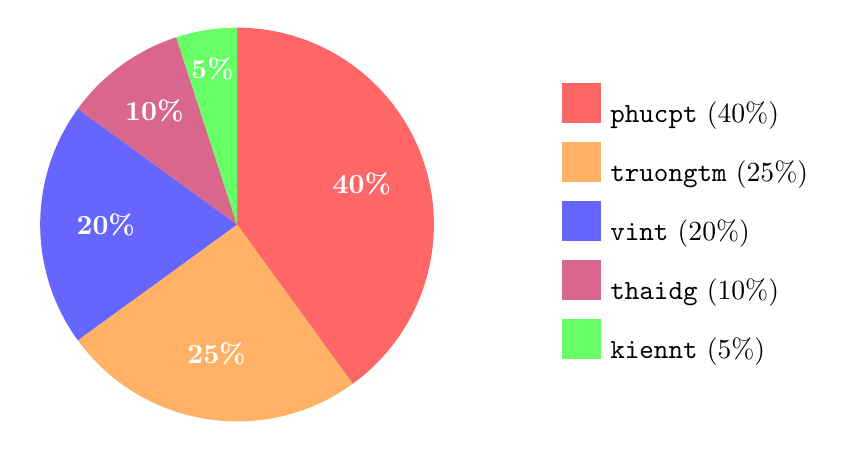
\begin{tikzpicture}
        % Vẽ biểu đồ tròn bằng TIKZ dựa trên góc tính toán từ % thực tế
        % 40% = 144 độ | 25% = 90 độ | 20% = 72 độ | 10% = 36 độ | 5% = 18 độ
        \def\radius{2.5cm}
        
        % phucpt: 40% (Từ 90 đến -54)
        \fill[red!60] (0,0) -- (90:\radius) arc (90:-54:\radius) -- cycle;
        % truongtm: 25% (Từ -54 đến -144)
        \fill[orange!60] (0,0) -- (-54:\radius) arc (-54:-144:\radius) -- cycle;
        % vint: 20% (Từ -144 đến -216)
        \fill[blue!60] (0,0) -- (-144:\radius) arc (-144:-216:\radius) -- cycle;
        % thaidg: 10% (Từ -216 đến -252)
        \fill[purple!60] (0,0) -- (-216:\radius) arc (-216:-252:\radius) -- cycle;
        % kiennt: 5% (Từ -252 đến -270 / tương đương 90 độ của vòng tiếp theo)
        \fill[green!60] (0,0) -- (-252:\radius) arc (-252:-270:\radius) -- cycle;
        
        % Chú thích % trên biểu đồ
        \node[text=white, font=\bfseries] at (18:\radius/1.5) {40\%};
        \node[text=white, font=\bfseries] at (-99:\radius/1.5) {25\%};
        \node[text=white, font=\bfseries] at (-180:\radius/1.5) {20\%};
        \node[text=white, font=\bfseries] at (-234:\radius/1.4) {10\%};
        \node[text=white, font=\bfseries] at (-261:\radius/1.25) {5\%};
        
        % Legend
        \node[anchor=west] at (4, 1.5) {\textcolor{red!60}{\rule{0.5cm}{0.5cm}} \texttt{phucpt} (40\%)};
        \node[anchor=west] at (4, 0.75) {\textcolor{orange!60}{\rule{0.5cm}{0.5cm}} \texttt{truongtm} (25\%)};
        \node[anchor=west] at (4, 0) {\textcolor{blue!60}{\rule{0.5cm}{0.5cm}} \texttt{vint} (20\%)};
        \node[anchor=west] at (4, -0.75) {\textcolor{purple!60}{\rule{0.5cm}{0.5cm}} \texttt{thaidg} (10\%)};
        \node[anchor=west] at (4, -1.5) {\textcolor{green!60}{\rule{0.5cm}{0.5cm}} \texttt{kiennt} (5\%)};
\end{tikzpicture}

% Biểu đồ 4: Biểu đồ tròn - Tỉ lệ Tài liệu/Source code
\begin{tikzpicture}
        \def\radius{2.5cm}
        
        % Tính toán xấp xỉ tổng cộng 233 commits
        % ~.tex commits: ~66 (28%) -> Góc: 101 độ
        % Non-.tex commits: ~167 (72%) -> Góc: 259 độ
        
        % Non-.tex: 72% (Từ 90 đến -169)
        \fill[blue!50] (0,0) -- (90:\radius) arc (90:-169:\radius) -- cycle;
        % .tex: 28% (Từ -169 đến -270 / tương đương 90 độ của vòng tiếp)
        \fill[orange!50] (0,0) -- (-169:\radius) arc (-169:-270:\radius) -- cycle;
        
        % Chú thích %
        \node[text=white, font=\bfseries] at (-39:\radius/1.5) {72\%};
        \node[text=white, font=\bfseries] at (140:\radius/1.5) {28\%};
        
        % Legend
        \node[anchor=west] at (4, 0.5) {\textcolor{blue!50}{\rule{0.5cm}{0.5cm}} Mã nguồn \texttt{game} Commits (72\%)};
        \node[anchor=west] at (4, -0.5) {\textcolor{orange!50}{\rule{0.5cm}{0.5cm}} \texttt{Tài liệu báo cáo} Commits (28\%)};
\end{tikzpicture}

\end{document}